% !TeX root = ../main.tex

\chapter{系统需求分析及架构设计}
本章节系统全面介绍了支持大规模高并发、实时反映表决情况的债权人会议系统的需求分析及架构设计工作。本章节从系统业务出发,分析了债权人会议系统的需求,根据需求进行了针对性的架构设计,说明了与原会议系统的区别之处并简单介绍了数据库设计和非实时后端设计。

\section{需求分析}

会议系统根据功能性质划分,分为两个大的模块,一是会议管理模块,另一个是会议系统主模块。运营平台会议管理模块负责会议的创建、修改及数据导入等会议管理功能。会议系统主模块负责视频直播、投票表决、实时查看数据、实时聊天等会议核心功能。

\subsection{会议管理模块}

会议系统管理模块负责会议管理相关的功能,会议的管理模块由运营人员在运营平台进行操作,运营人员具有的功能权限有创建/修改会议、导入表决数据、导入其他参会人员信息、获取密码反馈、激活会议、发送短信通知及获取推流地址。会议系统管理模块的具体功能需求如图~\ref{fig:meetingManagement} 所示。

\begin{figure}[!htp]
  \centering
  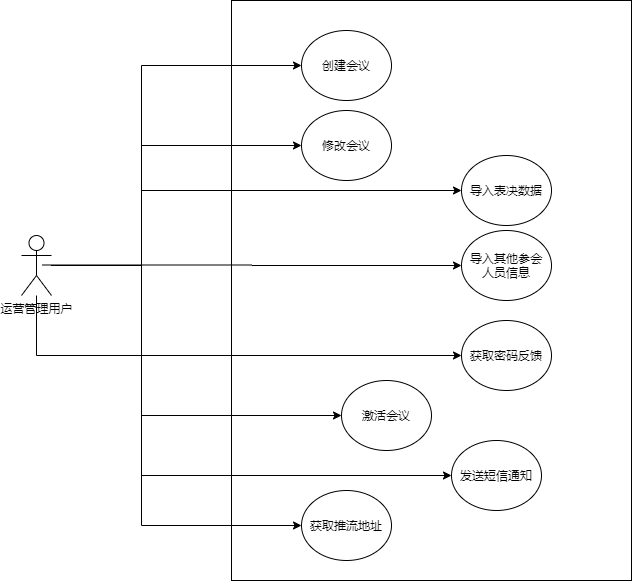
\includegraphics{meetingManagement.png}
  \caption[管理模块]
    {会议系统管理模块需求用例图}
 \label{fig:meetingManagement}
\end{figure}

\subsubsection{创建和修改会议}
原系统会议模块创建和修改会议分为三步,填写会议基本信息、填写议题相关信息、导入议题表决信息。导入议题表决信息显然和创建会议属于不同功能,将导入信息作为创建会议的一环并不合理,因此将导入议题表决信息功能单独拆出。另外将创建会议拆分成两步并没有实际意义,反而增加了创建会议时出现错误的概率,因此将填写会议基本信息、填写议题相关信息合并为一步。

运营管理人员在运营平台创建和修改会议。创建和修改会议需要填写会议的基本信息(会议名称和会议召开日期为必填项)、会议的议程信息(包括需表决和无需表决议程)、议程的表决组信息,由于向 OSS 文件系统存储会议文件和议程文件时,需要会议号作为索引,因此在创建会议前需要提前向后端请求获取预约会议号。

\subsubsection{导入表决数据和其他参会人员信息}
表决数据包括表决信息(表决所在表决组、表决金额等)和表决信息对应的债权人信息。原系统会议模块导入表决数据是创建会议的第三步,表决数据仅可导入原债权申报系统中已存在的数据,若仅使用会议功能,表决数据的导入和原债权申报系统数据强绑定的设计就显得极为不合理。因此将导入表决数据和原债权申报系统数据解除绑定,增加使用 Excel 文件上传导入表决数据。点击下载 Excel 模板,填写完表决数据完整信息后,点击导入表决数据上传填好的 Excel 文件。此时,可能存在债权人未在会议平台注册的情况,表决数据若对应已存在债权人,则将表决数据划分给已存在债权人。表决数据若对应不存在债权人,则先创建对应债权人,再将表决数据划给创建的债权人。

会议除相关管理人和债权人外,还存在其他参会人员(仅可观看会议)。其他参会人员不可自行注册,仅可通过运营人员在运营平台通过上传 Excel 文件导入,目的是为了防止会议无关人员参与会议。

\subsubsection{发送短信通知}
与原系统会议模块相比,还增加了自主短信群发通知功能。运营平台管理员可以向所有会议相关人员发送短信通知。选定模板和发送范围后,可以向指定范围发送会议相关信息。

\subsection{会议系统主模块}

原系统会议模块用户分为两类。一是管理人用户,二是债权人用户。若存在仅可观看会议的其他类型参会人员,需注册为债权人用户,不赋予表决数据,即可满足只能观看的需求。这种做法不符合规范,因此新增游客用户类型,仅提供观看会议的权限。

会议系统主模块负责会议的核心功能。债权人会议系统的用户分为三类。一是管理人用户,二是债权人用户,三是游客用户(即其他参会人员)。管理人用户具有开启表决、结束表决、查看表决详情、查看参会详情、设定结束日期、查看会议详情、查看会议列表、观看视频直播、实时聊天的功能。债权人用户具有签到、补签、投票表决、实时聊天、查看会议列表、查看会议详情、观看视频直播的功能。游客用户具有查看会议列表、查看会议详情、观看视频直播的功能。会议系统主模块的具体功能需求如图~\ref{fig:meetingMain} 所示。

会议系统主模块功能根据是否有实时性要求又分为实时模块和非实时模块。实时模块包括实时聊天功能和投票表决功能。

\begin{figure}[!htp]
  \centering
  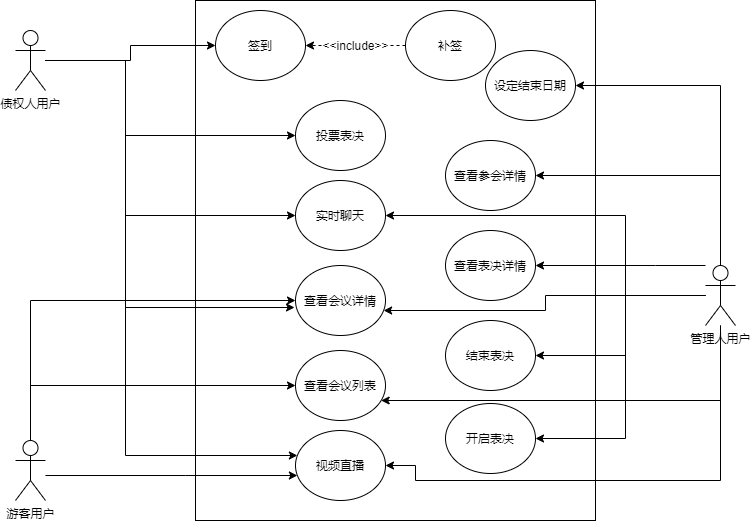
\includegraphics[width=14cm]{meetingMain.png}
  \caption[主模块]
    {会议系统主模块需求用例图}
 \label{fig:meetingMain}
\end{figure}

\subsubsection{开启和结束表决}
原系统会议模块的表决开启和结束由创建会议时设定的开启日期和结束日期决定,由于实际需求中,会议的表决开启和结束有时需要管理人进行控制,因此管理人用户增加了开启和结束表决的功能。

\subsubsection{查看参会详情和表决详情}
原系统会议模块仅有参看表决详情功能。在实际的会议中,管理人有时需要向法院报告会议参会情况,因此管理人用户增加了查看参会详情的功能,且在开会期间,表决相关数据均改为实时刷新。

\subsubsection{签到和补签}
原系统会议模块中,债权人参加会议功能在任何时间都可以使用,即时会议已经结束,债权人仍可点击参会,这与常理不符。现在改为债权人在会议开始到会议结束之间第一次进入会议时,会主动弹出签到框,提醒债权人签到参会,并提供补签功能,签到成功后才可进行投票表决。

\section{架构设计}
在破产领域中,债权人会议和表决的意义十分重大,决定着一个破产项目的走向。在一次实际的债权人会议中,债权人的数量级平均为千人级别,有些会议的债权人数量甚至可以达到上万人。债权人会议的一项重要工作是进行表决。在实际的会议中,表决可能在较短的时间内进行,因此会导致在短时间内出现大量请求。当同时有多个会议进行时,短时间激增的请求会给服务器带来极大的压力,因此需要针对性的设计架构应对此问题。

\subsection{现有架构及问题}

\subsubsection{现有架构}
\begin{figure}[!htp]
  \centering
  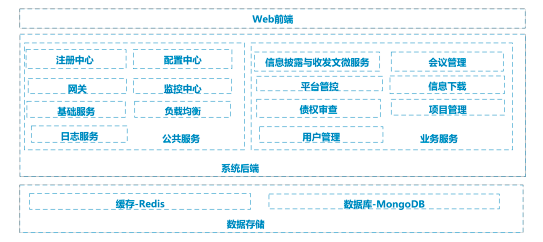
\includegraphics[width=12cm]{oldMeeting_1.png}
  \caption[原微服务]
    {原系统微服务架构图\cite{Wang2021}}
 \label{fig:oldMeeting_1}
\end{figure}

原系统采用微服务架构的原因一是原系统已具有比较完整
的服务治理管理体系,采用微服务架构将节省部署运维和降低系统升级的工作难度。这样
就能充分复用原系统的实现,减少开发系统,升级系统的成本。二是可以满足系统可
扩展性的要求。当需要对系统持续升级与优化时,可以直接设计其他微服务加入到微
服务治理体系中以满足用户不断扩展的需求。具体架构如图~\ref{fig:oldMeeting_1}\cite{Wang2021} 所示。根据微服务架构设计的高内聚低耦合的原则,原系统将会议管理整体划分为一个微服务,所有会议相关的功能全部集中放在会议管理微服务中。

在原系统的设计中,当用户数上升时,可以为各个微服
务起多个实例同时服务来满足用户并发数,可以在不改变软件架构的基础上通
过增加硬件资源来提高服务质量。

\begin{figure}[!htp]
  \centering
  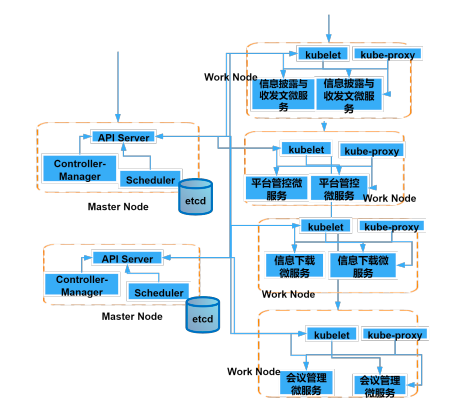
\includegraphics[height=8cm]{oldMeeting_2.png}
  \caption[原物理架构]
    {原系统物理架构图\cite{Wang2021}}
 \label{fig:oldMeeting_2}
\end{figure}

原系统是在 k8s 集群上进行部署的,系统采用图~\ref{fig:oldMeeting_2}
的物理架构。系统用户可以直接通过浏览器访问系统。而用户的请求都将到达 K8s 集群中
的 Mater Node,由 Master Node 结点进行处理。Mater Node 结点是整个集群的管理结点,该
结点会根据请求的特性命令 Work Node 结点进行作业工作。另外,一个服务往往运行成多个实例以增加系统的容错性。


\nocite{Wang2021}
\subsubsection{存在问题}
本文主要针对原系统的两个重要问题进行改善,一个是会议进行过程中的实时性不强,一个是无法保证在高并发情况下可以完成正常的服务。

高并发情况下本系统能够正常运行需要对架构进行设计以应对高压力情况。对债权人会议来讲,可能发生高并发的情况有两种:

1. 多个会议同时进行时,大量债权人在短时间内发送多条消息,造成大量请求涌向服务器

2. 多个会议同时进行时,大量债权人在短时间内进行表决,造成大量请求涌向服务器

在原系统的实现中,会议管理微服务实现为 SpringBoot 后端,在会议管理微服务中通过 WebSocket 实现实时聊天,通过轮询实现管理人查询数据的实时更新。

首先,假设系统需要能同时处理 200 场会议,每个会议债权人数量为 1000 人,仅仅实时聊天的长链接数量就达到了 20 万级别。SpringBoot 项目的默认启动容器是 Tomcat,而 Tomcat 默认支持的连接数量为 1 万,这个数量级远远低于要求。按照原系统设计为会议管理微服务起多个实例同时服务来满足并发数需要启动接近 20 个实例,这仅仅是为了满足保持实时聊天的长连接数量。

其次,原系统通过轮询方式实现管理人端查看数据的实时更新,这会给服务器带来较大的压力,且比较浪费资源,债权人侧投票表决和管理人侧数据实时刷新也应当通过 WebScoket 实现。

会议进行过程中数据的实时刷新本文通过对实时服务进行设计解决,将在第三章进行详细讲述,下面将介绍本系统如何针对高并发带来的问题进行设计解决问题。

\subsection{架构设计}
原聊天服务通过 Tomcat 启动连接数过低,无法支持高并发,而考虑到为了支持大量实时请求时可以更快更好的扩充聊天服务实例,并且实时聊天服务可以不仅针对会议系统使用,考虑到其功能和扩展性,考虑将实时聊天服务单独实现为一个微服务,并且实时服务不使用 SpringBoot 项目实现,而是通过 Golang 实现,不使用 Tomcat 作为启动容器,大大提升了其单个实例连接数上限。同样考虑到应对高并发情况,实时表决服务也实现为一个单独的微服务。

对债权人会议来讲,高并发情况主要针对实时服务,即上面划分出的实时聊天服务和实时表决服务。在高并发情况下,如果直接将数据全部持久化到 MongoDB 数据库, Mongo 写入不及时可能导致读取的数据并非理想情况下的最新数据,带来数据一致性问题。为了保证在高并发时的数据一致性,本系统考虑使用 Redis 集群作为高速缓存,因为高并发情况仅仅存在于会议进行期间,会议持续时间并不长,因此在会议开始时,将会议所有相关实体存入 Redis 集群,在会议进行期间数据的读取来自于 Redis 集群中,数据的写入会先更新 Redis 集群中的数据,更新成功后将向非实时后端发送请求,将数据持久化至 Mongo 数据库。为了防止高并发时实时服务向非实时服务发送的请求过多导致非实时服务后端崩溃,本系统选择使用 Kafka 集群用作流量削峰,实施服务通过生产者生产一条需要写回数据库的消息,通过 Kafka 集群的发布订阅功能,非实时后端的消费者消费此条消息,将数据持久化到 Mongo 集群。

\begin{figure}[!htp]
  \centering
  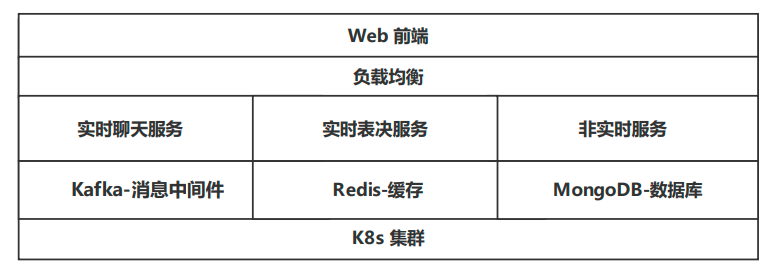
\includegraphics[width=12cm]{cluster.png}
  \caption[实时微服务架构]
    {债权人会议系统架构图}
 \label{fig:cluster}
\end{figure}

针对系统的某个实时微服务,如表决服务、聊天服务,所有用户均使用同一套服务架构。
该服务架构一定包括无状态的 WebSocket 服务实例集群,以及独立的有状态 Redis 集群。Redis 集群是实例的状态中心,存储实例的所有状态数据。

本系统将原本的会议管理微服务拆分为非实时服务(除去实时功能)、实时表决微服务和实时聊天微服务。新的非实时服务包含会议除去实时部分的所有相关功能(创建会议等),与原本实现差别不大。会议开始前和会议结束后的表决数据查询通过非实时服务,而在会议进行中时,表决数据查询通过实时微服务进行,本文后端的主要设计针对实时服务设计,非实时服务后端和数据库设计不是本文重点,仅在本章进行简单的介绍。

\section{数据库设计}

本会议系统的后端涉及到的角色有四种,一是运营人员,二是管理人,三是债权人,四是其他参会人员。涉及到的主要功能有会议基本信息的增删改查、会议的数据导入(包括表决数据导入和其他参会人员信息导入)、直播服务、实时聊天室、实时表决服务等。根据是否和实时性相关将本系统的后端主要分为两个部分,一是非实时服务部分的后端,实现为 SpringBoot 后端; 二是实时服务部分的后端,用 Golang 实现为 WebSocket 后端。

需要持久化到 Mongo 数据库的数据结构全部存在于非实时服务后端,因此数据库设计仅展示非实时服务后端的数据库设计。

如图~\ref{fig:meetingER}所示,整个系统的数据实体被划分为 Meeting, Schedule,
Group, Ticket, MeetingCreditor, ChatRoom 这 6 种类型的实体以满足需求。其中 Meeting 表示会议, Schedule 表示议程, Group 表示表决组, Ticket 表示选票, ChatRoom 表示会议聊天室。

\begin{figure}[!htp]
    \centering
    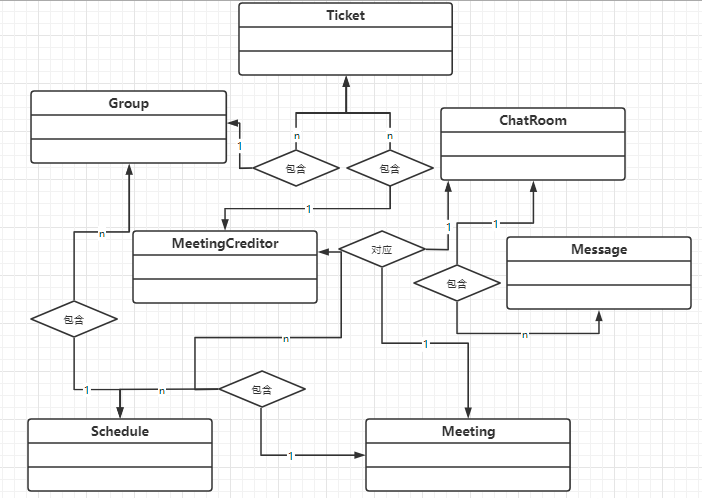
\includegraphics[width=14cm]{meetingER.png}
    \caption{会议系统数据库 ER 图}
    \label{fig:meetingER}
  \end{figure}

本系统使用 Meeting、Schedule、Group 数据实体满足会议信息管理的需求,他们分别表示了会议的基本信息,会议议程信息,议程表决组信息。Meeting 包含了会议的会议名称、创建时间、案件编号以及对应的聊天室 id 等基础信息,Schedule 包含了议程的名称,对应的会议 id ,议程的类型等信息, Group 包含了表决组名称,对应的议程 id 等信息。MeetingCreditor 满足了会议债权人管理的需求,保存着代理人代理的会议债权人的信息。Ticket 满足了投票表决的需求,它包含了选票对应的会议债权人的 id ,对应的表决组 id ,对应的表决金额以及选票的赞成或反对等信息。 ChatRoom 和 Message 满足了实时聊天的需求,其中 Message 包含了所属聊天室 id ,消息内容,发送时间和接收人(接收者的用户 id,为空 null 或 [] 则为广播群发)等信息,聊天室包含聊天室的开启状态和禁用用户列表等信息。

\section{非实时后端设计与实现}
非实时后端包含了所有非实时性的功能,主要包括会议基本信息的增删改查、会议的数据导入(包括表决数据导入和其他参会人员信息导入)、其他参会人员登录及直播服务。


\subsection{会议基本信息管理的增删改查}
\subsubsection{创建和修改会议}
在原系统中议程被称为议题,下面统称议程。原系统会议模块创建和修改会议分为三步,分别是填写会议基本信息、填写议程相关信息、导入议程表决信息,只有三步全部完成会议才能创建成功,否则为暂存状态。原本的设计存在一些问题,一是会议创建分为三步过于累赘,导入议程表决信息并不属于创建会议的工作。二是会议和表决强绑定,仅含有无表决议程的会议无法通过导入议程表决信息这一步。

基于以上问题,对创建和修改会议进行了调整。一是将填写会议基本信息和填写议程相关信息合并为一步。在实际实现的时候发现创建会议时,在创建会议请求发送以前,就需要获取会议 id 用于存储会议文件和议程文件至 OSS 文件系统对应会议 id 目录下,因此在创建会议前需要先获取会议 id 。本系统会议的 id 号由 Redis 数据库存储的对应 id 控制,因此在创建会议前,先向 Redis 预约一个会议 id, 在创建会议时将对应会议文件和议程文件存至 OSS文件系统对应目录下,由于从 Redis 中获取 id 后,设置了 id 自增,因此会议 id 号预约唯一。并且由于创建会议时,有多个实体需要存至Mongo数据库,因此实现方法时添加了SpringBoot 的事务性注解,一旦创建会议失败,回滚所有数据库操作。二是将导入议程表决信息从创建修改会议中拆出,仅含有无表决议程的会议也可以正常创建会议,而导入议程表决信息仅有含有需表决议程且导入标记为 false 的会议需要进行,通过这样的设计,仅无表决议程的会议可以正常完成流程。

\subsubsection{删除会议}
原系统会议模块中,删除会议为直接从数据库中删除对应会议全部数据,由于需要规避误删及恶意删除的情况以及需要提供删除恢复的功能,直接从数据库中删除数据的方式不可取,本系统删除操作全部改为采用逻辑删除,对应实体添加 deleted 字段用以表示对应数据是否被删除,为 true 则表示该数据已被删除。

\subsubsection{查询会议}
和原系统会议模块相比,查询会议功能主要有两个重要的变化。一是由于新系统删除操作全部改为逻辑删除,因此在查询时需要根据 deleted 字段进行筛选,获取未被删除的数据。二是原系统会议模块会议的状态是通过获取会议列表事件进行驱动的,在每次获取会议列表时,会对获取到的会议进行一次处理,根据会议召开时间和当前服务器时间的对比重新更新会议状态。在每次获取会议列表时,都会进行这样的操作,假设有 1000 个人拥有1个同样的会议,他们每个人获取一次会议列表,这个会议的状态都会被更新1000遍,即这个会议会被重新存储1000次,如果短时间内大量的人获取会议列表,且每个人会议列表包含的会议数量都不少的情况下,服务器的资源可能很快就被耗尽,这是不可取的。会议的状态仅仅是前端展示的一个维度,不需要存入数据库,只要在获取会议列表时通过会议召开时间和当前服务器时间的对比设置返回给前端的会议状态字段即可。

\subsection{会议系统的数据导入}
会议系统的数据导入分为两个部分,一是表决数据导入,二是其他参会人员信息导入。

原系统的表决数据导入为直接从债权审查模块拉取审查数据,如果用户仅仅使用会议系统而不使用债权审查,会议就无法获取相关数据,会议无法正常进行。这种情况下,会议系统和债权审查系统就变成了强绑定关系,而这是不合理的。因此需要新增额外的导入手段,本系统使用的导入方式是Excel模板导入的方式。用户先从前端点击下载表决数据导入的模板,在填入对应信息后上传表决数据表格,非实时服务后端通过逐条读取表决数据表格,导入相关表决信息,若代理人或会议债权人不存在,还需要通过表中信息自动创建代理人和会议债权人,多次导入时,如果对应选票数据存在则进行复用,表中有但数据库中无对应数据的进行创建操作,剩余的上一次导入数据全部逻辑删除,所有存储操作在导入模板数据全部读取完成后进行,若读取发现模板存在错误,则此次导入数据不存回数据库,并将错误信息通过Excel表格返回给用户。表决信息模板如表~\ref{fig:meetingImport}所示。

\begin{table}[h!]
    \begin{center}
      \caption{表决信息导入模板}
      \label{fig:meetingImport}
      \begin{tabular}{c c c c c c }
        \hline
        \textbf{债权人名称} & \textbf{编号} & \textbf{债权所在表决组} & \textbf{表决金额} & \textbf{参会人姓名} & \textbf{参会人手机号} \\
        \hline
        \\
        \hline
      \end{tabular}
    \end{center}
  \end{table}

本系统由于除开参与会议管理的管理人和行使表决权利的债权人外,还有一些其他的参会人员,如法官、无表决权债权人等,只参观会议的进行,不参与其他操作。为了更好地区分,额外设置了其他参会人员,其他参会人员的信息在表决信息导入后,也通过 Excel 表格进行导入,导入方式同表决信息导入,其他参会人员仅参观会议,实际上只在会议进行期间有效,因此其他参会人员信息存入 Redis,无需持久化到 Mongo 数据库,一旦会议结束即可删除。导入其他参会人员信息模板如表~\ref{fig:otherUserImport}所示。

\begin{table}[h!]
    \begin{center}
      \caption{其他参会人员信息导入模板}
      \label{fig:otherUserImport}
      \begin{tabular}{ c c c }
        \hline
       \textbf{参会人姓名} & \textbf{参会人手机号} & \textbf{参会人类型} \\
       \hline
       \\
       \hline
      \end{tabular}
    \end{center}
  \end{table}

在实现了导入后,由于导入模板中存在的新的代理人和会议债权人为系统自动创建,密码也由系统自动创建,而 user 后端的数据加密方式为非对称加密,无法通过数据库中存储的加密 password 字段反向获取明文的密码,因此需要提供自动生成密码的反馈给用户,由于导入可以重复进行,若将密码生成放在导入时,可能会重复进行多次生成密码,这样变相产生浪费。因此改为信息导入都成功后,点击生成密码则会调用生成密码接口自动为对新创建的代理人和会议债权人创建密码,并将生成的密码导出至 Excel 返回并将密码在 OSS文件系统中备份,如果需要再次获取密码,则点击生成密码反馈,直接向 OSS 文件系统请求获取生成密码的 Excel 备份文件。生成密码反馈 Excel 如表~\ref{fig:passwordReturn}所示。

\begin{table}[h!]
    \begin{center}
      \caption{密码反馈模板}
      \label{fig:passwordReturn}
      \begin{tabular}{ c c c c c }
        \hline
       \textbf{用户名称} & \textbf{手机号(登录账号)} & \textbf{密码} & \textbf{用户类型} & \textbf{代理债权人名单} \\
       \hline
       \\
       \hline
      \end{tabular}
    \end{center}
  \end{table}

  \subsection{其他参会人员登录}
  前面提到其他参会人员实际只在会议召开期间有效,且信息不会持久化到 Mongo 数据库,如果使用密码登录,显得比较累赘,因此考虑使用其他登录方式。首先考虑的是使用游客链接登录的方式,直接向其他参会人员发送可以参会的游客链接,点击即可入会参会。管理人反馈使用链接登录和使用账号密码登录对于管理人通知来说是两种参会方式,要减轻管理人的负担,应该让代理人可以通过一致、统一的方式登录,方便管理人沟通,且使用管理人认为链接可以随意转发,会议安全性无法保证。

  游客登录方案不可行,参考目前各系统通用的登录方式后决定使用手机号验证码登录的方式,既可以保证安全性,又不需存储其他参会人员的密码,方便快捷。其他参会人员使用验证码登录时,在 sms 后端生成验证码并通过阿里云短信服务接口向对应手机号发送短信,获得成功反馈后将验证码存至 Redis, 其他参会人员填写发送登录验证请求后,向Redis获取验证码进行对比,若验证码仍在15分钟有效期内,且登录验证码和Redis所存验证码相符合,则登录成功并将 Redis中存储的对应验证码清除。

  \subsection{直播服务}

  \begin{figure}[!htp]
    \centering
    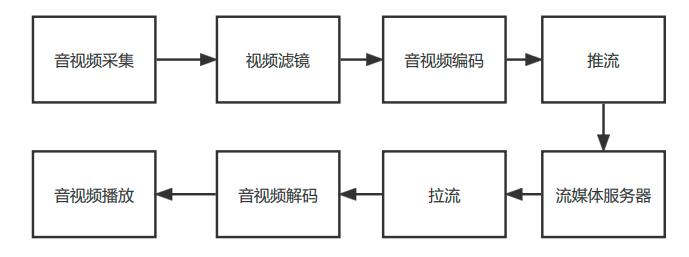
\includegraphics[height=5cm,width=14cm]{live.png}
    \caption{直播服务流程示意图}
    \label{fig:live}
  \end{figure}

  如图~\ref{fig:live}所示,目前直播服务的流程都是先进行音视频采集,然后进行视频的滤镜转换,转换后进行音视频编码,将编码好的音视频推流至流媒体服务器,播放端向流媒体服务器进行拉流,然后对拉取的流进行音视频解码,最后播放。目前本系统直播服务音视频采集、视频滤镜、音视频编码、推流的方式是通过摄像机采集音视频、控制滤镜,音视频编码和推流通过美菲特 M3803 编码器编码并推流。
  流媒体服务器使用的是阿里云直播服务,前端向后端发送请求,后端通过 API 向阿里云直播服务获取拉流地址。

  在使用过程中发现,单一推拉流不够稳定,在长时间的直播中可能出现断线的情况,这对债权人会议来讲是不可接受的,为了解决这个问题,本系统采取了多路推流的方式,同时将一个直播流向多个推流地址进行推流,当一个推流地址出现问题时,可以通过切换线路保证直播服务的质量。

\section{本章小结}
本章首先对支持大规模高并发、实时反映表决情况的债权人会议系统的需求进行了分析,将会议系统分为了管理模块和主模块两部分,分别画出了会议系统的需求用例图,并对新系统和原系统在功能需求上的差异做出了对比并说明了原因。在需求分析完毕之后,本章先介绍了原系统的架构设计,说明了原先架构存在的问题并针对现有会议功能需求,给出了针对性的架构设计,并简单介绍了系统数据库设计和非实时部分后端的设计实现。